The Spot Trace data from the Java Sea and Makassar Strait snapper fisheries illustrate that management by WPP is sometimes impossible. In the case of the snapper fisheries in WPP 712 and WPP 713, many vessels fish right at the border, often fishing in both these WPP even within single fishing trips. Also landings made at ports in any specific WPP, are not necessarily fish caught in that particular WPP, and this is especially true for snappers, groupers and emperors landed and processed in East Java, on the coast of WPP 712. The fish that is processed in major processing centers like Probolinggo comes from a number of different fleets that operate throughout the waters of Eastern Indonesian, including WPP 718 (Arafura Sea) and WPP 573 (Timor Sea).

\begin{center}
\graphicspath{{/root/R-project/IFishSnapperWPP712_713/Images/}}
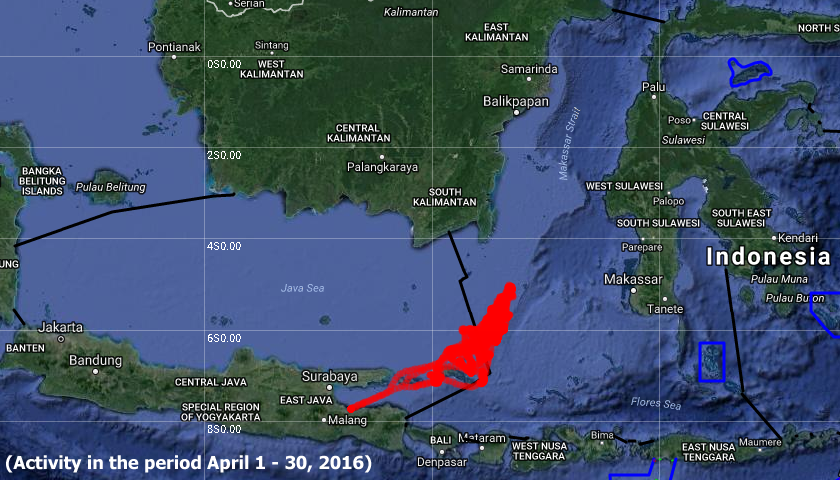
\includegraphics[width=15cm]{SpotTrace-712_713-April1-30_2016.png}

Figure 5. Tracks of long line and drop line fishing boats operating in the Java Sea (WPP 712) and the Makassar Strait (WPP 713).
\end{center}

\begin{center}
\graphicspath{{/root/R-project/IFishSnapperWPP712_713/Images/}}
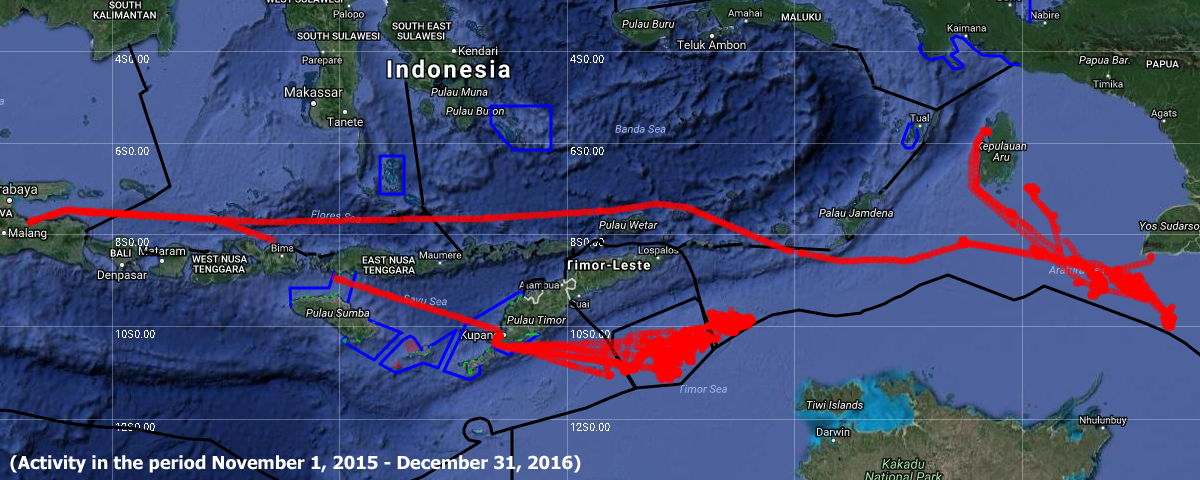
\includegraphics[width=15cm]{ProbolinggoFleetIn573_718_JPDA.png}

Figure 6. Tracks of long line fishing boats based in Probolingo, East Java, operating in the Timor Sea (WPP 573) and the Arafura Sea (WPP 718).
\end{center}


Potential IUU issues related to fish landed at ports in WPP 712 and 713 include the illegal operation by various fleets outside Indonesian waters in the East Timorese - Australian Joint Petroleum Development Area (JPDA). Fish from these waters may be mixed with fish from various Indonesian fisheries management areas, including WPP 712 and WPP 713, at the processing plants in Probolinggo. Additional issues include the under marking of medium scale vessels to below 30GT, the licensing of the various fleets for various WPP and the operation of fleets from remote ports inside Marine Protected Areas throughout Eastern Indonesia. All this needs to be discussed with fishing boat captains and boat owners to prevent issues of supply line ``pollution'' with IUU fish from thee protected areas.
